\documentclass[tikz,border=8pt]{standalone}
\usepackage[T1]{fontenc}
\usepackage{lmodern}
\usepackage{amsmath,amssymb}
\usepackage{pgfplots}
\pgfplotsset{compat=1.18}

\definecolor{navy}{RGB}{20,45,90}
\definecolor{crimson}{RGB}{175,30,45}
\definecolor{teal}{RGB}{0,125,120}
\definecolor{slate}{RGB}{110,125,145}

\begin{document}
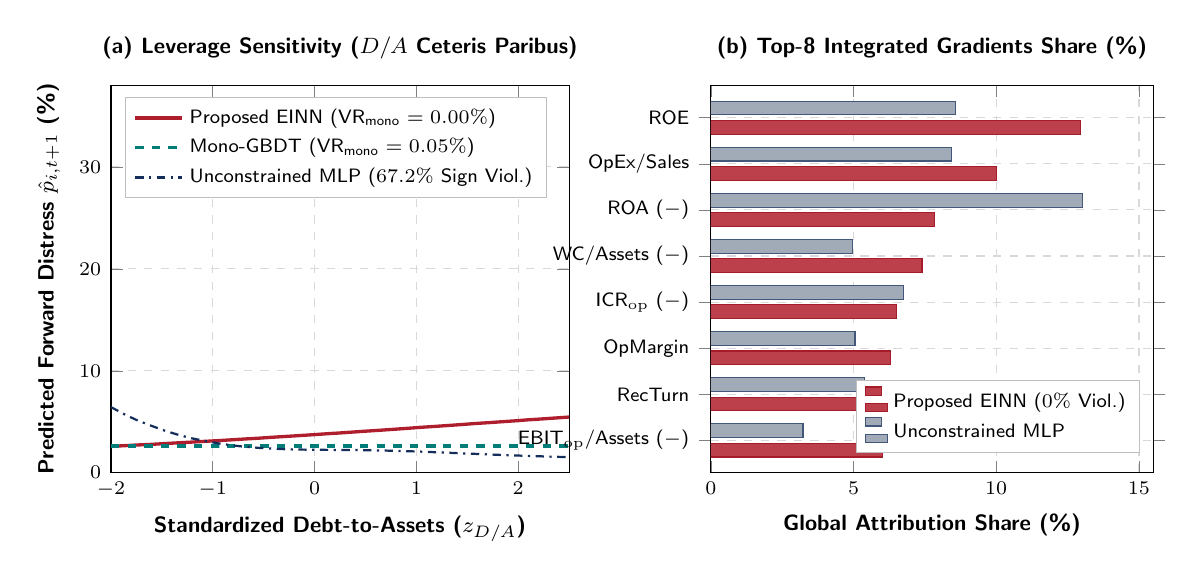
\begin{tikzpicture}
% Left Panel: Partial Dependence on Debt-to-Assets
\begin{axis}[
    name=panelA,
    width=7.4cm,
    height=6.5cm,
    title={\textbf{(a) Leverage Sensitivity ($D/A$ Ceteris Paribus)}},
    xlabel={\textbf{Standardized Debt-to-Assets ($z_{D/A}$)}},
    ylabel={\textbf{Predicted Forward Distress $\hat{p}_{i,t+1}$ (\%)}},
    xmin=-2.0, xmax=2.5,
    ymin=0, ymax=38,
    grid=both,
    grid style={dashed, gray!30},
    label style={font=\footnotesize\sffamily},
    title style={font=\footnotesize\sffamily},
    ticklabel style={font=\scriptsize},
    legend style={at={(0.03,0.97)}, anchor=north west, font=\scriptsize\sffamily, fill=white, draw=gray!50},
    legend cell align={left}
]
\addplot[color=crimson, very thick] coordinates {
    (-2.00,2.58) (-1.87,2.65) (-1.74,2.72) (-1.60,2.78) (-1.47,2.86) (-1.34,2.93) (-1.21,3.00) (-1.07,3.08) (-0.94,3.15) (-0.81,3.23) (-0.68,3.31) (-0.54,3.39) (-0.41,3.48) (-0.28,3.56) (-0.15,3.64) (-0.01,3.73) (0.12,3.82) (0.25,3.90) (0.38,3.99) (0.51,4.08) (0.65,4.17) (0.78,4.26) (0.91,4.35) (1.04,4.45) (1.18,4.54) (1.31,4.63) (1.44,4.72) (1.57,4.82) (1.71,4.91) (1.84,5.00) (1.97,5.09) (2.10,5.19) (2.24,5.28) (2.37,5.37) (2.50,5.46)
};
\addlegendentry{Proposed EINN ($\text{VR}_{\text{mono}}=0.00\%$)}

\addplot[color=teal, very thick, dashed] coordinates {
    (-2.00,2.62) (-1.87,2.62) (-1.74,2.62) (-1.60,2.62) (-1.47,2.62) (-1.34,2.62) (-1.21,2.62) (-1.07,2.62) (-0.94,2.62) (-0.81,2.62) (-0.68,2.62) (-0.54,2.62) (-0.41,2.62) (-0.28,2.62) (-0.15,2.62) (-0.01,2.62) (0.12,2.62) (0.25,2.62) (0.38,2.62) (0.51,2.62) (0.65,2.62) (0.78,2.62) (0.91,2.62) (1.04,2.62) (1.18,2.62) (1.31,2.62) (1.44,2.62) (1.57,2.62) (1.71,2.62) (1.84,2.62) (1.97,2.62) (2.10,2.62) (2.24,2.62) (2.37,2.62) (2.50,2.62)
};
\addlegendentry{Mono-GBDT ($\text{VR}_{\text{mono}}=0.05\%$)}

\addplot[color=navy, thick, dashdotted] coordinates {
    (-2.00,6.44) (-1.87,5.74) (-1.74,5.13) (-1.60,4.59) (-1.47,4.12) (-1.34,3.72) (-1.21,3.38) (-1.07,3.10) (-0.94,2.87) (-0.81,2.68) (-0.68,2.54) (-0.54,2.43) (-0.41,2.36) (-0.28,2.30) (-0.15,2.27) (-0.01,2.25) (0.12,2.24) (0.25,2.23) (0.38,2.22) (0.51,2.21) (0.65,2.18) (0.78,2.15) (0.91,2.11) (1.04,2.07) (1.18,2.01) (1.31,1.96) (1.44,1.90) (1.57,1.85) (1.71,1.79) (1.84,1.74) (1.97,1.69) (2.10,1.65) (2.24,1.60) (2.37,1.56) (2.50,1.53)
};
\addlegendentry{Unconstrained MLP ($67.2\%$ Sign Viol.)}
\end{axis}

% Right Panel: Top-8 Axiomatic Integrated Gradients Attribution Share
\begin{axis}[
    name=panelB,
    at={(panelA.east)}, anchor=west, xshift=1.8cm,
    xbar,
    bar width=5pt,
    width=7.2cm,
    height=6.5cm,
    title={\textbf{(b) Top-8 Integrated Gradients Share (\%)}},
    xlabel={\textbf{Global Attribution Share (\%)}},
    xmin=0, xmax=15.5,
    ytick={0,1,2,3,4,5,6,7},
    yticklabels={EBIT$_{\mathrm{op}}$/Assets ($-$),RecTurn,OpMargin,ICR$_{\mathrm{op}}$ ($-$),WC/Assets ($-$),ROA ($-$),OpEx/Sales,ROE},
    yticklabel style={font=\scriptsize\sffamily},
    xticklabel style={font=\scriptsize},
    label style={font=\footnotesize\sffamily},
    title style={font=\footnotesize\sffamily},
    grid=major,
    grid style={dashed, gray!30},
    legend style={at={(0.97,0.05)}, anchor=south east, font=\scriptsize\sffamily, fill=white, draw=gray!50},
    legend cell align={left}
]
\addplot[fill=crimson!85, draw=crimson!95!black] coordinates {
    (6.02,0) (6.11,1) (6.29,2) (6.49,3) (7.40,4) (7.84,5) (10.02,6) (12.95,7)
};
\addlegendentry{Proposed EINN ($0\%$ Viol.)}

\addplot[fill=slate!65, draw=navy!80] coordinates {
    (3.23,0) (5.39,1) (5.05,2) (6.75,3) (4.95,4) (13.03,5) (8.44,6) (8.57,7)
};
\addlegendentry{Unconstrained MLP}
\end{axis}
\end{tikzpicture}
\end{document}
